\documentclass [a4paper] {article}

\usepackage[utf8]{inputenc}


\title{\textbf{Práctica 2: Fundamentos de la ciencia de datos}}
\author{Luis Alejandro Cabanillas, Alvaro de las Heras, Mohssin Nagib Najim}

\usepackage{Sweave}
\begin{document}

\maketitle

\section{Ejercicio 1} En la primera parte se realizará un ejercicio en clase, con la ayuda del profesor, en el que se va a llevar a cabo un análisis
de las asociaciones de los datos en R. En este ejercicio tendremos un conjunto de 6 sucesos a modo de cestas de la compra. Los sucesos elementales que podemos
encontrarnos son {Pan}, {Agua}, {Leche}, {Naranjas} y {Café}.

La muestra que hemos obtenido consta de seis sucesos:
\begin{itemize}
	\item \textbf{{Pan, Agua, Leche, Naranjas}}
	\item \textbf{{Pan, Agua, Café, Leche}}
	\item \textbf{{Pan, Agua, Leche}}
        \item \textbf{{Pan, Café, Leche}}
        \item \textbf{{Pan, Agua}}
        \item \textbf{{Leche}}										 
\end{itemize}

\subsection{Instalación paquete arules} 
Para la realización del ejercicio necesitaremos el paquete arules, que implementa el algoritmo apriori y las reglas de asociación en R. 
Para ver si tenemos este paquete por defecto en R tendremos que ejecutar la siguiente instrucción:
\begin{Schunk}
\begin{Sinput}
> getOption("defaultPackages")
\end{Sinput}
\begin{Soutput}
[1] "datasets"  "utils"     "grDevices" "graphics"  "stats"     "methods"  
[7] "foreign"  
\end{Soutput}
\end{Schunk}

Como podemos ver, no tenemos el paquete por defecto en R, es decir, no tenemos el paquete cargado cada vez que se inicia R. Para comprobar
si tenemos instalado el paquete, ejecutamos el siguiente comando:
\begin{Schunk}
\begin{Sinput}
> library()
\end{Sinput}
\end{Schunk}
Tenemos el paquete instalado; por lo que tenemos que cargarlo en el entorno actual:
\begin{Schunk}
\begin{Sinput}
> library(arules)
\end{Sinput}
\end{Schunk}

Si no tuviésemos el paquete instalado, tenemos que seguir los siguientes pasos:
\begin{itemize}
	\item \textbf{1. Ir a la página web de CRAN Project.}: En la página de CRAN Project se puede acceder a los paquetes, que se pueden encontrar 
                                                                																					ordenados por nombre. Cada paquete incluye los archivos binario y un manual de referencia.
	\item \textbf{2. Descargar el archivo binario y el manual de referencia}: En este caso descargaremos la versión 1.6-4 del paquete.
	\item \textbf{3. Ejecutar la orden en R para instalar el paquete}: Debemos ejecutar install.packages("ruta del paquete").
    \item \textbf{4. Cargar el paquete en R}: Con la instrucción vista anteriormente en este documento library(arules).									 
\end{itemize}

Una vez tenemos el paquete instalado y cargado, podemos realizar el ejercicio.

\subsection{Introducción de los datos de la muestra en R} 
Lo primero que tenemos que hacer es introducir la muestra en una matriz, para poder trabajar con ella. En la matriz introduciremos unos y ceros en función de cada 
suceso:
\begin{Schunk}
\begin{Sinput}
> muestra <- Matrix(c(1,1,0,1,1,1,1,1,1,0,1,1,0,1,0,1,0,1,1,0,1,1,0,0,0,0,0,0,1,0),
+ 6,5,byrow=T,dimnames=list(c("suceso1","suceso2","suceso3","suceso4","suceso5","suceso6"),
+ c("Pan","Agua","Cafe","Leche","Naranjas")),sparse=T)
> muestra
\end{Sinput}
\begin{Soutput}
6 x 5 sparse Matrix of class "dgCMatrix"
        Pan Agua Cafe Leche Naranjas
suceso1   1    1    .     1        1
suceso2   1    1    1     1        .
suceso3   1    1    .     1        .
suceso4   1    .    1     1        .
suceso5   1    1    .     .        .
suceso6   .    .    .     1        .
\end{Soutput}
\end{Schunk}
Ya tenemos la matriz con la muestra, a continuación deberemos prepararla para su análisis. 
Para ello, la pasaremos a un formato nsparse y haremos la transpuesta:
\begin{Schunk}
\begin{Sinput}
> muestraNGCMatrix <- as(muestra,"nsparseMatrix")
> transpmuestraNGCMatrix <- t(muestraNGCMatrix)
> transpmuestraNGCMatrix
\end{Sinput}
\begin{Soutput}
5 x 6 sparse Matrix of class "ngCMatrix"
         suceso1 suceso2 suceso3 suceso4 suceso5 suceso6
Pan            |       |       |       |       |       .
Agua           |       |       |       .       |       .
Cafe           .       |       .       |       .       .
Leche          |       |       |       |       .       |
Naranjas       |       .       .       .       .       .
\end{Soutput}
\end{Schunk}

Ahora deberemos convertir esta matriz en una serie de transacciones para poder ser usada por el algoritmo apriori. 
Estas transacciones se corresponden a cada uno de los sucesos: Se pasan los ceros y unos a variables con el ID del suceso:
\begin{Schunk}
\begin{Sinput}
> transacciones <- as(transpmuestraNGCMatrix,"transactions")
> transacciones
\end{Sinput}
\begin{Soutput}
transactions in sparse format with
 6 transactions (rows) and
 5 items (columns)
\end{Soutput}
\begin{Sinput}
> inspect(transacciones)
\end{Sinput}
\begin{Soutput}
    items                     itemsetID
[1] {Pan,Agua,Leche,Naranjas} suceso1  
[2] {Pan,Agua,Cafe,Leche}     suceso2  
[3] {Pan,Agua,Leche}          suceso3  
[4] {Pan,Cafe,Leche}          suceso4  
[5] {Pan,Agua}                suceso5  
[6] {Leche}                   suceso6  
\end{Soutput}
\end{Schunk}

Para ver datos estadísticos básicos sobre nuestros datos usamos el comando summary():
\begin{Schunk}
\begin{Sinput}
> summary(transacciones)
\end{Sinput}
\begin{Soutput}
transactions as itemMatrix in sparse format with
 6 rows (elements/itemsets/transactions) and
 5 columns (items) and a density of 0.5666667 

most frequent items:
     Pan    Leche     Agua     Cafe Naranjas  (Other) 
       5        5        4        2        1        0 

element (itemset/transaction) length distribution:
sizes
1 2 3 4 
1 1 2 2 

   Min. 1st Qu.  Median    Mean 3rd Qu.    Max. 
  1.000   2.250   3.000   2.833   3.750   4.000 

includes extended item information - examples:
  labels
1    Pan
2   Agua
3   Cafe

includes extended transaction information - examples:
  itemsetID
1   suceso1
2   suceso2
3   suceso3
\end{Soutput}
\end{Schunk}

\subsection{Aplicación del algoritmo apriori}
Una vez tenemos los datos introducidos en R, ya podemos aplicar el algoritmo apriori para ver las asociaciones. Para aplicar este algoritmo deberemos 
usar la instrucción apriori(datos,parameter=list(support=umbral de soporte,confidance=umbral de confianza)).

Así, lo aplicamos sobre nuestros datos:
\begin{Schunk}
\begin{Sinput}
> asociaciones <- apriori(transacciones,parameter=list(support=0.5,confidence=0.8))
\end{Sinput}
\begin{Soutput}
Apriori

Parameter specification:
 confidence minval smax arem  aval originalSupport maxtime support minlen
        0.8    0.1    1 none FALSE            TRUE       5     0.5      1
 maxlen target   ext
     10  rules FALSE

Algorithmic control:
 filter tree heap memopt load sort verbose
    0.1 TRUE TRUE  FALSE TRUE    2    TRUE

Absolute minimum support count: 3 

set item appearances ...[0 item(s)] done [0.00s].
set transactions ...[5 item(s), 6 transaction(s)] done [0.00s].
sorting and recoding items ... [3 item(s)] done [0.00s].
creating transaction tree ... done [0.00s].
checking subsets of size 1 2 3 done [0.00s].
writing ... [7 rule(s)] done [0.00s].
creating S4 object  ... done [0.00s].
\end{Soutput}
\begin{Sinput}
> asociaciones
\end{Sinput}
\begin{Soutput}
set of 7 rules 
\end{Soutput}
\begin{Sinput}
> inspect(asociaciones)
\end{Sinput}
\begin{Soutput}
    lhs             rhs     support   confidence lift count
[1] {}           => {Leche} 0.8333333 0.8333333  1.00 5    
[2] {}           => {Pan}   0.8333333 0.8333333  1.00 5    
[3] {Agua}       => {Pan}   0.6666667 1.0000000  1.20 4    
[4] {Pan}        => {Agua}  0.6666667 0.8000000  1.20 4    
[5] {Leche}      => {Pan}   0.6666667 0.8000000  0.96 4    
[6] {Pan}        => {Leche} 0.6666667 0.8000000  0.96 4    
[7] {Agua,Leche} => {Pan}   0.5000000 1.0000000  1.20 3    
\end{Soutput}
\end{Schunk}

Podemos concluir que las asociaciones que cumplen los umbrales establecidos son 5.

\section{Ejercicio 2} En esta segunda parte se nos pide desarrollar dos ejercicios, el primero consistirá en aplicar el procedimiento
que se realizó en el ejercicio 1 para otros datos de muestra leídos desde un fichero .txt y la segunda parte consistira en desarrollar un
enunciado y la solución de este realizando el analisis con R de asociación.

\subsubsection{Análisis de datos muestra extras de coches} 
En este ejercicio se nos pide, a partir de un .txt generado según los datos de muestra proporcionados
en el enunciado sobre los extras que puede llevar un coche, resolver utilizando el algoritmo Apriori y obtener las asociaciones
cuyo soporte sea igual o superior al 40% y cuya confianza sea igual o superior al 90%.

Lo primero que haremos será cargar los datos del .txt que hemos generado a partir de los datos proporcionados en el enunciado, para esto
utilizaremos el read.table organizándolo como una matriz. Los sucesos elementales que podemos
encontrarnos son {X:Faros de Xenon}, {A: Alarma}, {T: Techo Solar}, {N: Navegador}, {B: Bluetooth} y {C: Control de Crucero}.

La muestra que hemos obtenido consta de ocho sucesos:
\begin{itemize}
	\item \textbf{{X, C, N, B}}
	\item \textbf{{X, T, B, C}}
	\item \textbf{{N, C, X}}
        \item \textbf{{N, T, X, B}}
        \item \textbf{{X, C, B}}
        \item \textbf{{N}}		
		\item \textbf{{X, B, C}}	
		\item \textbf{{T, A}}									 
\end{itemize}

\begin{Schunk}
\begin{Sinput}
> extras<-as.matrix(read.table("extras.txt"))
> extras
\end{Sinput}
\begin{Soutput}
  X A T N B C
1 1 0 0 1 1 1
2 1 0 1 0 1 1
3 1 0 0 1 0 1
4 1 0 1 1 1 0
5 1 0 0 0 1 1
6 0 0 0 1 0 0
7 1 0 0 0 1 1
8 0 1 1 0 0 0
\end{Soutput}
\end{Schunk}

Al importar los datos vemos que se nos genera una matriz pero esta es de tipo lista por lo que tendremos que convertirla en matriz:
\begin{Schunk}
\begin{Sinput}
> extrasM<-Matrix(extras, sparse=T)
> extrasM
\end{Sinput}
\begin{Soutput}
8 x 6 sparse Matrix of class "dgCMatrix"
  X A T N B C
1 1 . . 1 1 1
2 1 . 1 . 1 1
3 1 . . 1 . 1
4 1 . 1 1 1 .
5 1 . . . 1 1
6 . . . 1 . .
7 1 . . . 1 1
8 . 1 1 . . .
\end{Soutput}
\end{Schunk}

Ahora pasaremos la matriz a matriz de patron dispersa:
\begin{Schunk}
\begin{Sinput}
> extrasNGC<-as(extrasM, "nsparseMatrix")
> extrasNGC
\end{Sinput}
\begin{Soutput}
8 x 6 sparse Matrix of class "ngCMatrix"
  X A T N B C
1 | . . | | |
2 | . | . | |
3 | . . | . |
4 | . | | | .
5 | . . . | |
6 . . . | . .
7 | . . . | |
8 . | | . . .
\end{Soutput}
\end{Schunk}

Posteriormente sacaremos la traspuesta de la matriz generada anteriormente para sacar las transacciones:
\begin{Schunk}
\begin{Sinput}
> transpExtras <- t(extrasNGC)
> transpExtras
\end{Sinput}
\begin{Soutput}
6 x 8 sparse Matrix of class "ngCMatrix"
  1 2 3 4 5 6 7 8
X | | | | | . | .
A . . . . . . . |
T . | . | . . . |
N | . | | . | . .
B | | . | | . | .
C | | | . | . | .
\end{Soutput}
\begin{Sinput}
> transacciones<-as(transpExtras, "transactions")
> transacciones
\end{Sinput}
\begin{Soutput}
transactions in sparse format with
 8 transactions (rows) and
 6 items (columns)
\end{Soutput}
\end{Schunk}

Podemos ver el numero de transacciones en filas y el numero de items que tenemos en columnas.

Mostramos las estadísticas de las transacciones con summary, datos como los elementos más frecuentes, la distribucion
del tamaño de los elementos, el minimo, la mediana y la media, entre otros:
\begin{Schunk}
\begin{Sinput}
> summary(transacciones)
\end{Sinput}
\begin{Soutput}
transactions as itemMatrix in sparse format with
 8 rows (elements/itemsets/transactions) and
 6 columns (items) and a density of 0.5 

most frequent items:
      X       B       C       N       T (Other) 
      6       5       5       4       3       1 

element (itemset/transaction) length distribution:
sizes
1 2 3 4 
1 1 3 3 

   Min. 1st Qu.  Median    Mean 3rd Qu.    Max. 
   1.00    2.75    3.00    3.00    4.00    4.00 

includes extended item information - examples:
  labels
1      X
2      A
3      T

includes extended transaction information - examples:
  itemsetID
1         1
2         2
3         3
\end{Soutput}
\end{Schunk}

\subsubsection{Aplicación del algoritmo apriori}

Aplicamos el algoritmo apriori para calcular las asociaciones, con un soporte de un 40 por ciento o superior y una confianza de un 80 por ciento o superior:
\begin{Schunk}
\begin{Sinput}
> asociaciones<-apriori(transacciones,parameter=list(support=0.4, confidence=0.9))
\end{Sinput}
\begin{Soutput}
Apriori

Parameter specification:
 confidence minval smax arem  aval originalSupport maxtime support minlen
        0.9    0.1    1 none FALSE            TRUE       5     0.4      1
 maxlen target   ext
     10  rules FALSE

Algorithmic control:
 filter tree heap memopt load sort verbose
    0.1 TRUE TRUE  FALSE TRUE    2    TRUE

Absolute minimum support count: 3 

set item appearances ...[0 item(s)] done [0.00s].
set transactions ...[6 item(s), 8 transaction(s)] done [0.00s].
sorting and recoding items ... [4 item(s)] done [0.00s].
creating transaction tree ... done [0.00s].
checking subsets of size 1 2 3 done [0.00s].
writing ... [3 rule(s)] done [0.00s].
creating S4 object  ... done [0.00s].
\end{Soutput}
\begin{Sinput}
> inspect(asociaciones)
\end{Sinput}
\begin{Soutput}
    lhs      rhs support confidence lift     count
[1] {C}   => {X} 0.625   1          1.333333 5    
[2] {B}   => {X} 0.625   1          1.333333 5    
[3] {B,C} => {X} 0.500   1          1.333333 4    
\end{Soutput}
\end{Schunk}

Podemos ver que las asociaciones que cumplen las condiciones de soporte y confianza son 3.

\subsection{Ejercicio 2.2}
En este ejercicio el objetivo será encontrar las asociaciones de un conjunto de recetas, este conjunto de datos lo hemos obtenido en Kaggle.com. 
La idea es encontrar que ingredientes se usan y como se asocian, siendo una modificación del típico problema de las cestas pero con datos reales,
para ello emplearemos la biblioteca de \textbf{arules} junto \textbf{arulesViz} (visualización) y \textbf{jsonlite}  para la lectura.
\begin{Schunk}
\begin{Sinput}
> install.packages("jsonlite")
> library("jsonlite")
> install.packages("arules")
> library("arules")
> install.packages("arulesViz")
> library("arulesViz")
\end{Sinput}
\end{Schunk}
Una vez instaladas y cargadas las bibliotecas hay que cargar nuestros datos, en este caso como es un JSON usaremos \textbf{readjson()} de jsonlite, sobre estos
datos seleccionaremos el de los ingredientes, que es el que de verdad nos interesa.
\subsubsection{Carga y preparación de los datos}
\begin{Schunk}
\begin{Sinput}
> json<-read_json("Ingredientes.json", simplifyVector=TRUE)
> datos <- json$ingredients
\end{Sinput}
\end{Schunk}
Para dotar de mayor informacion a los datos le añadimos un ID que será el futuro ID de la transacción, para ello utilizamos \textbf{names()} para asignar valores a
los nombres de los objetos (set) y \textbf{paste()} para generar una cadena de texto a partir de los vectores que generamos. Además como añadido hemos creado una 
función para asignar un tipo aleatorio que será una variable cualitativa, con 5 posibles valores. Dentro de la función se usan vectores, números aleatorios enteros
generados con \textbf{sample()} y el método \textbf{append()} para concatenar elementos al vector. Sin embargo, a diferencia del caso anterior añadiremos estos datos de forma distinta
y después de haber creado las transacciones.
\begin{Schunk}
\begin{Sinput}
> names(datos ) <- paste("receta-",c(1:length(datos )), sep = "")
> tipo <- function(d){
+     categorias <- c("mala","mediocre","normal","buena","recomendable")
+     tipos <- c()
+     for (i in 1:length(d)){
+         n_aleatorio <-sample(1:length(categorias), 1)
+         v<-categorias [n_aleatorio]
+         tipos <- append(tipos,v)
+     }
+     tipos 
+ }
\end{Sinput}
\end{Schunk}
Con los datos ya listos el siguiente paso es crear las transacciones que se hace usando el método \textbf{as()} junto al parametro "transactions", al ser una entrada compatible (list)
lo realiza sin problema. Con las transacciones creadas le asignamos ahora los datos que habíamos creado antes, modificando la información de las transacciones con la función
\textbf{transactionInfo()}, en la que indicamos la transacción y el nombre de la columna. Como podemos observar la información y transacciones son correctas.
\begin{Schunk}
\begin{Sinput}
> transacciones <- as(datos, "transactions")
> transactionInfo(transacciones)[["tipo"]] <- tipo(datos)
> transactionInfo(head(transacciones ,5))
\end{Sinput}
\begin{Soutput}
  transactionID         tipo
1      receta-1 recomendable
2      receta-2       normal
3      receta-3       normal
4      receta-4        buena
5      receta-5         mala
\end{Soutput}
\begin{Sinput}
> inspect(head(transacciones ,5))
\end{Sinput}
\begin{Soutput}
    items                             transactionID         tipo
[1] {all-purpose flour,                                         
     baking powder,                                             
     eggs,                                                      
     milk,                                                      
     raisins,                                                   
     white sugar}                          receta-1 recomendable
[2] {bananas,                                                   
     corn starch,                                               
     cream of tartar,                                           
     egg whites,                                                
     egg yolks,                                                 
     light rum,                                                 
     milk,                                                      
     sugar,                                                     
     toasted pecans,                                            
     vanilla extract,                                           
     vanilla wafers}                       receta-2 normal      
[3] {cuban peppers,                                             
     fennel bulb,                                               
     fronds,                                                    
     olive oil,                                                 
     onions,                                                    
     sausage links}                        receta-3 normal      
[4] {all-purpose flour,                                         
     andouille sausage,                                         
     boneless chicken skinless thigh,                           
     browning,                                                  
     dried thyme,                                               
     file powder,                                               
     flat leaf parsley,                                         
     freshly ground pepper,                                     
     garlic cloves,                                             
     ham,                                                       
     hot sauce,                                                 
     lump crab meat,                                            
     meat cuts,                                                 
     okra,                                                      
     paprika,                                                   
     shrimp,                                                    
     smoked sausage,                                            
     vegetable oil,                                             
     water,                                                     
     white rice,                                                
     yellow onion}                         receta-4 buena       
[5] {cornmeal,                                                  
     extra-virgin olive oil,                                    
     ground black pepper,                                       
     leeks,                                                     
     parmigiano reggiano cheese,                                
     salt,                                                      
     sausage casings,                                           
     water}                                receta-5 mala        
\end{Soutput}
\end{Schunk}
\begin{Schunk}
\begin{Sinput}
> image(transacciones )
\end{Sinput}
\end{Schunk}
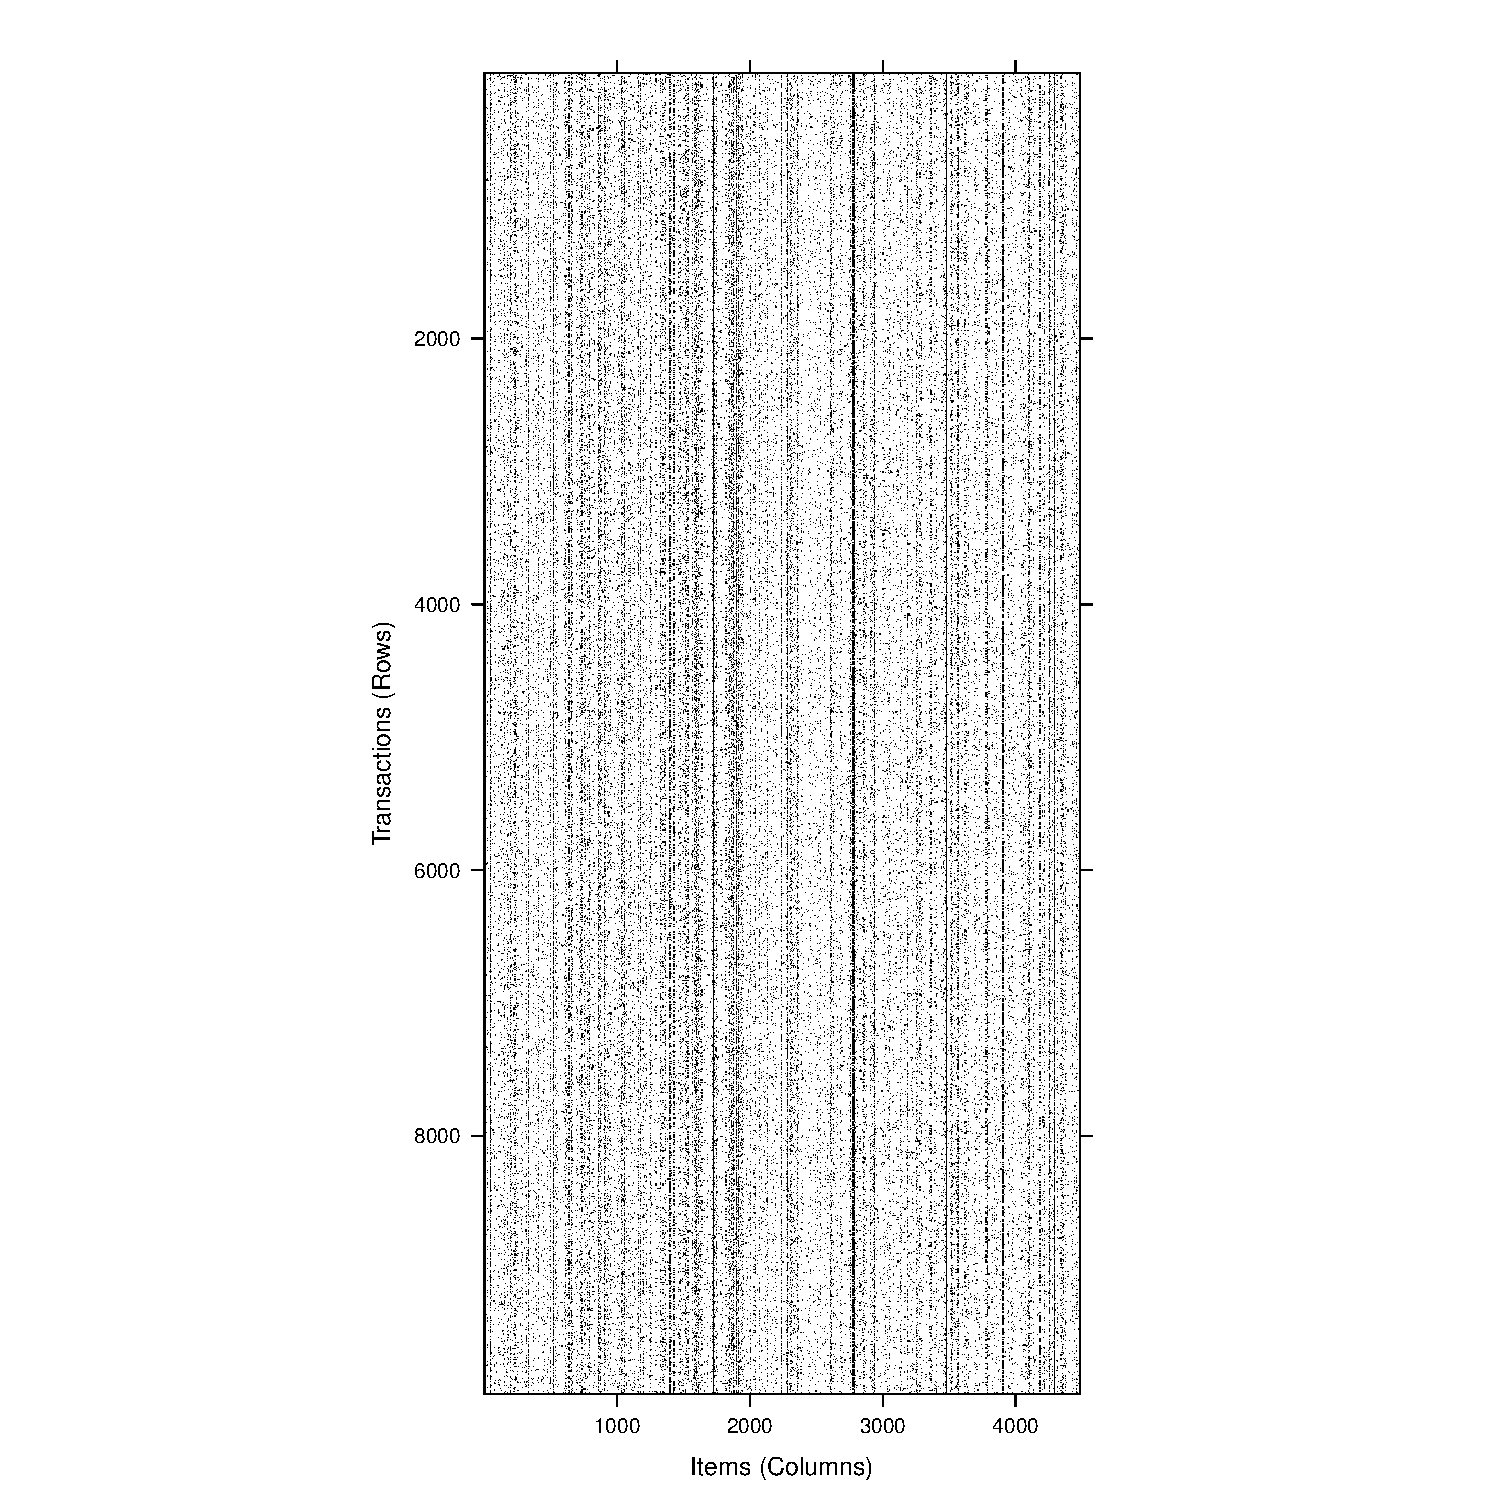
\includegraphics{Practica2-transacciones}
\subsubsection{Algoritmos para la búsqueda asociaciones}
A partir de las transacciones ahora es posible aplicar los distintos algoritmos para obtener las relaciones, a los que asignaremos distintos valores de confianza y soporte.
El primer algoritmo que aplicaremos es el apriori, en el que a partir de una serie de pasos obtiene relaciones candidatas según un soporte y después una confianza, cuyo valores
definirán la fuerza de la asociación. En este caso solo hay que introducir el soporte y la confianza.
\begin{Schunk}
\begin{Sinput}
> asociaciones <- apriori(transacciones , parameter= list(support=0.05, confidence=0.3))
\end{Sinput}
\begin{Soutput}
Apriori

Parameter specification:
 confidence minval smax arem  aval originalSupport maxtime support minlen
        0.3    0.1    1 none FALSE            TRUE       5    0.05      1
 maxlen target   ext
     10  rules FALSE

Algorithmic control:
 filter tree heap memopt load sort verbose
    0.1 TRUE TRUE  FALSE TRUE    2    TRUE

Absolute minimum support count: 497 

set item appearances ...[0 item(s)] done [0.00s].
set transactions ...[4484 item(s), 9944 transaction(s)] done [0.04s].
sorting and recoding items ... [24 item(s)] done [0.01s].
creating transaction tree ... done [0.00s].
checking subsets of size 1 2 3 done [0.00s].
writing ... [15 rule(s)] done [0.00s].
creating S4 object  ... done [0.00s].
\end{Soutput}
\begin{Sinput}
> inspect(asociaciones)
\end{Sinput}
\begin{Soutput}
     lhs                      rhs         support    confidence lift     count
[1]  {}                    => {salt}      0.45102574 0.4510257  1.000000 4485 
[2]  {pepper}              => {salt}      0.09271923 0.8616822  1.910495  922 
[3]  {butter}              => {salt}      0.07290829 0.5894309  1.306868  725 
[4]  {all-purpose flour}   => {salt}      0.07743363 0.6503378  1.441908  770 
[5]  {vegetable oil}       => {salt}      0.05380129 0.4730327  1.048793  535 
[6]  {ground black pepper} => {salt}      0.06667337 0.5502075  1.219903  663 
[7]  {sugar}               => {salt}      0.07693081 0.4693252  1.040573  765 
[8]  {garlic cloves}       => {olive oil} 0.05168946 0.3348534  1.736976  514 
[9]  {garlic cloves}       => {salt}      0.07662912 0.4964169  1.100640  762 
[10] {water}               => {salt}      0.09945696 0.5386710  1.194324  989 
[11] {olive oil}           => {salt}      0.10488737 0.5440793  1.206315 1043 
[12] {garlic}              => {onions}    0.06667337 0.3701843  1.808012  663 
[13] {onions}              => {garlic}    0.06667337 0.3256385  1.808012  663 
[14] {garlic}              => {salt}      0.09332261 0.5181463  1.148818  928 
[15] {onions}              => {salt}      0.11122285 0.5432220  1.204415 1106 
\end{Soutput}
\end{Schunk}
Si modificamos los parametros que reciben podemos seleccionar los tamaños de las transacciones quitando así las reglas con antecedentes vacíos (implican la aparación de esos objetos sin tener en cuenta otros).
También si queremos tener más precisión podemos seleccionar que valores queremos tener a la izquierda o derecha de la relacion. Como se observa en
el resultado hay pocas asociaciones que pasen el soporte que es relativamente bajo, esto quiere decir que las asociaciones no son fuertes, la razón de esto 
se debe a que el conjunto de datos engloba una gran cantidad de diversas recetas, con platos de distintas culturas y tipos como puede ser la repostería.
\begin{Schunk}
\begin{Sinput}
> asociaciones <- apriori(transacciones , parameter= list(minlen=2, support=0.05, confidence=0.3))
\end{Sinput}
\begin{Soutput}
Apriori

Parameter specification:
 confidence minval smax arem  aval originalSupport maxtime support minlen
        0.3    0.1    1 none FALSE            TRUE       5    0.05      2
 maxlen target   ext
     10  rules FALSE

Algorithmic control:
 filter tree heap memopt load sort verbose
    0.1 TRUE TRUE  FALSE TRUE    2    TRUE

Absolute minimum support count: 497 

set item appearances ...[0 item(s)] done [0.00s].
set transactions ...[4484 item(s), 9944 transaction(s)] done [0.05s].
sorting and recoding items ... [24 item(s)] done [0.00s].
creating transaction tree ... done [0.00s].
checking subsets of size 1 2 3 done [0.00s].
writing ... [14 rule(s)] done [0.00s].
creating S4 object  ... done [0.00s].
\end{Soutput}
\begin{Sinput}
> inspect(asociaciones)
\end{Sinput}
\begin{Soutput}
     lhs                      rhs         support    confidence lift     count
[1]  {pepper}              => {salt}      0.09271923 0.8616822  1.910495  922 
[2]  {butter}              => {salt}      0.07290829 0.5894309  1.306868  725 
[3]  {all-purpose flour}   => {salt}      0.07743363 0.6503378  1.441908  770 
[4]  {vegetable oil}       => {salt}      0.05380129 0.4730327  1.048793  535 
[5]  {ground black pepper} => {salt}      0.06667337 0.5502075  1.219903  663 
[6]  {sugar}               => {salt}      0.07693081 0.4693252  1.040573  765 
[7]  {garlic cloves}       => {olive oil} 0.05168946 0.3348534  1.736976  514 
[8]  {garlic cloves}       => {salt}      0.07662912 0.4964169  1.100640  762 
[9]  {water}               => {salt}      0.09945696 0.5386710  1.194324  989 
[10] {olive oil}           => {salt}      0.10488737 0.5440793  1.206315 1043 
[11] {garlic}              => {onions}    0.06667337 0.3701843  1.808012  663 
[12] {onions}              => {garlic}    0.06667337 0.3256385  1.808012  663 
[13] {garlic}              => {salt}      0.09332261 0.5181463  1.148818  928 
[14] {onions}              => {salt}      0.11122285 0.5432220  1.204415 1106 
\end{Soutput}
\begin{Sinput}
> buscamosSal <- apriori(transacciones , parameter= list(support=0.1, confidence=0.1),appearance = list(default="lhs",rhs="salt"))
\end{Sinput}
\begin{Soutput}
Apriori

Parameter specification:
 confidence minval smax arem  aval originalSupport maxtime support minlen
        0.1    0.1    1 none FALSE            TRUE       5     0.1      1
 maxlen target   ext
     10  rules FALSE

Algorithmic control:
 filter tree heap memopt load sort verbose
    0.1 TRUE TRUE  FALSE TRUE    2    TRUE

Absolute minimum support count: 994 

set item appearances ...[1 item(s)] done [0.00s].
set transactions ...[4484 item(s), 9944 transaction(s)] done [0.04s].
sorting and recoding items ... [12 item(s)] done [0.00s].
creating transaction tree ... done [0.01s].
checking subsets of size 1 2 done [0.00s].
writing ... [3 rule(s)] done [0.00s].
creating S4 object  ... done [0.00s].
\end{Soutput}
\begin{Sinput}
> tenemosSal <- apriori(transacciones , parameter= list(support=0.1, confidence=0.1, minlen=2),appearance = list(default="rhs",lhs="salt"))
\end{Sinput}
\begin{Soutput}
Apriori

Parameter specification:
 confidence minval smax arem  aval originalSupport maxtime support minlen
        0.1    0.1    1 none FALSE            TRUE       5     0.1      2
 maxlen target   ext
     10  rules FALSE

Algorithmic control:
 filter tree heap memopt load sort verbose
    0.1 TRUE TRUE  FALSE TRUE    2    TRUE

Absolute minimum support count: 994 

set item appearances ...[1 item(s)] done [0.00s].
set transactions ...[4484 item(s), 9944 transaction(s)] done [0.04s].
sorting and recoding items ... [12 item(s)] done [0.00s].
creating transaction tree ... done [0.00s].
checking subsets of size 1 2 done [0.00s].
writing ... [2 rule(s)] done [0.00s].
creating S4 object  ... done [0.00s].
\end{Soutput}
\begin{Sinput}
> inspect(sort(buscamosSal ))
\end{Sinput}
\begin{Soutput}
    lhs            rhs    support   confidence lift     count
[1] {}          => {salt} 0.4510257 0.4510257  1.000000 4485 
[2] {onions}    => {salt} 0.1112228 0.5432220  1.204415 1106 
[3] {olive oil} => {salt} 0.1048874 0.5440793  1.206315 1043 
\end{Soutput}
\begin{Sinput}
> inspect(sort(tenemosSal ))
\end{Sinput}
\begin{Soutput}
    lhs       rhs         support   confidence lift     count
[1] {salt} => {onions}    0.1112228 0.2465998  1.204415 1106 
[2] {salt} => {olive oil} 0.1048874 0.2325530  1.206315 1043 
\end{Soutput}
\end{Schunk}
Arules además del algoritmo apriori implementa el algoritmo eclat y su variante weclat. Este algoritmo busca los objetos más frecuentes pero lo hace de forma más eficiente y escalable que el apriori.
Su funcionamiento se basa en el método de búsqueda en profundidad frente a la búsqueda en anchura que ofrece el apriori, comenzando primero con los subsets más pequeños y aumentando hasta que no se puedan formar más.
Además, nosotros hemos aplicado una versión similar en la que hemos aplicado pesos a cada transacción, teniendo en cuenta esos pesos en la búsqueda de candidatos. En este caso solo es necesario introducir el soporte, aunque
se pueden introducir más parámetros, después podremos ver los valores y las imágenes. Con los candidatos generados solo queda aplicar \textbf{ruleInduction()} para generar las reglas de asociación. El resultado será el mismo que 
el del algoritmo apriori con la diferencia del ahorro en coste, especialmente si trabajamos con muchos datos como ahora, pero Sweave no soporta tantos datos por lo que hemos cambiado el soporte.
\begin{Schunk}
\begin{Sinput}
> # Asociaciones por Eclat
> candidatosECLAT <- eclat(transacciones ,parameter = list(support = 0.1, tidLists = TRUE))
\end{Sinput}
\begin{Soutput}
Eclat

parameter specification:
 tidLists support minlen maxlen            target   ext
     TRUE     0.1      1     10 frequent itemsets FALSE

algorithmic control:
 sparse sort verbose
      7   -2    TRUE

Absolute minimum support count: 994 

create itemset ... 
set transactions ...[4484 item(s), 9944 transaction(s)] done [0.04s].
sorting and recoding items ... [12 item(s)] done [0.00s].
creating bit matrix ... [12 row(s), 9944 column(s)] done [0.00s].
writing  ... [14 set(s)] done [0.00s].
Creating S4 object  ... done [0.00s].
\end{Soutput}
\begin{Sinput}
> inspect(sort(candidatosECLAT ))
\end{Sinput}
\begin{Soutput}
     items                 support   count
[1]  {salt}                0.4510257 4485 
[2]  {onions}              0.2047466 2036 
[3]  {olive oil}           0.1927796 1917 
[4]  {water}               0.1846340 1836 
[5]  {garlic}              0.1801086 1791 
[6]  {sugar}               0.1639179 1630 
[7]  {garlic cloves}       0.1543644 1535 
[8]  {butter}              0.1236927 1230 
[9]  {ground black pepper} 0.1211786 1205 
[10] {all-purpose flour}   0.1190668 1184 
[11] {vegetable oil}       0.1137369 1131 
[12] {onions,salt}         0.1112228 1106 
[13] {pepper}              0.1076026 1070 
[14] {olive oil,salt}      0.1048874 1043 
\end{Soutput}
\begin{Sinput}
> asociacionesECLAT <- ruleInduction(candidatosECLAT , confidence = 0.3)
> inspect(asociacionesECLAT )
\end{Sinput}
\begin{Soutput}
    lhs            rhs    support   confidence lift    
[1] {olive oil} => {salt} 0.1048874 0.5440793  1.206315
[2] {onions}    => {salt} 0.1112228 0.5432220  1.204415
\end{Soutput}
\end{Schunk}
\begin{Schunk}
\begin{Sinput}
> image(tidLists(candidatosECLAT ))
\end{Sinput}
\end{Schunk}
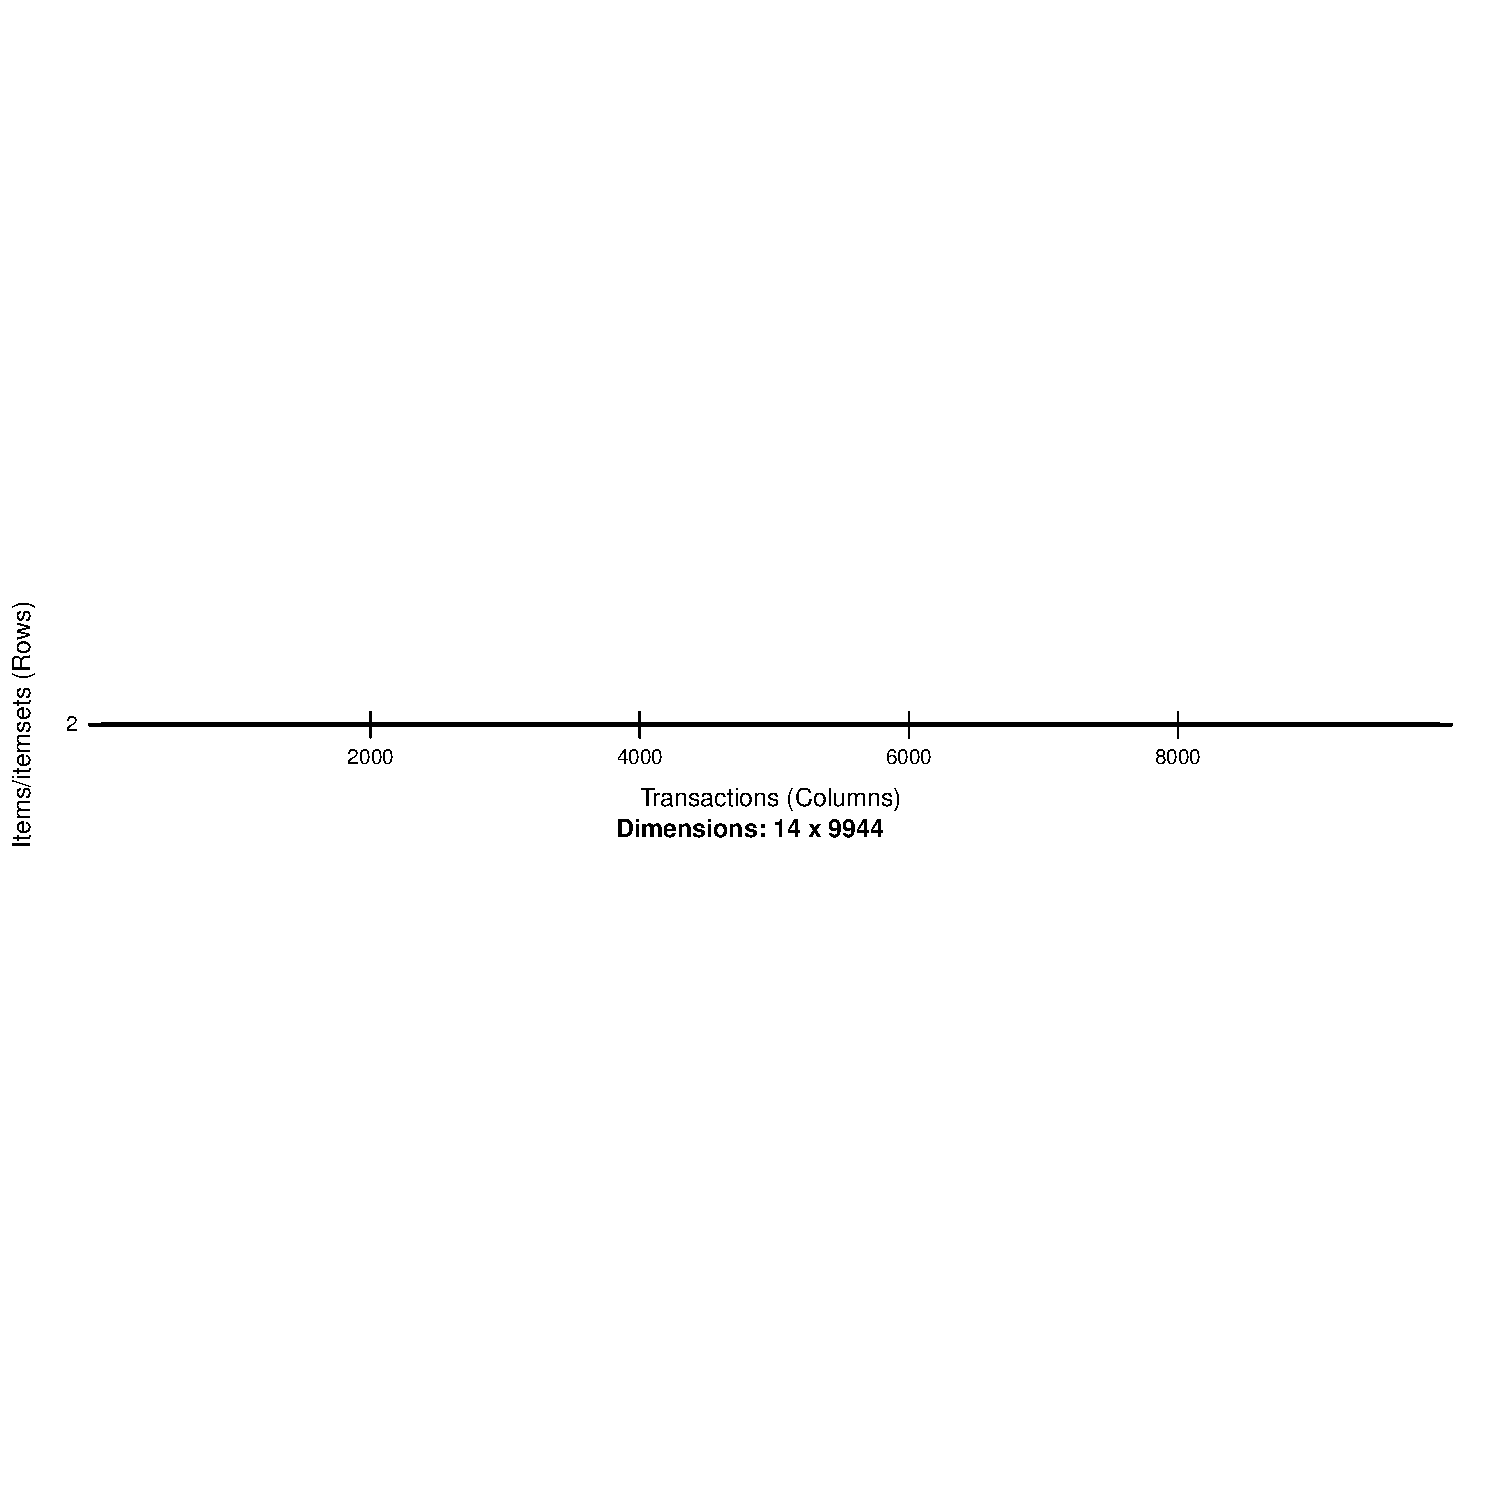
\includegraphics{Practica2-candEclat}
\begin{Schunk}
\begin{Sinput}
> # Asociaciones por Weclat (Eclat con pesos)
> pesos <- runif(length(transacciones), 0.0, 1.0)
> transactionInfo(transacciones)[["weight"]] <- pesos
> inspect(head(transacciones ,5) )
\end{Sinput}
\begin{Soutput}
    items                             transactionID         tipo     weight
[1] {all-purpose flour,                                                    
     baking powder,                                                        
     eggs,                                                                 
     milk,                                                                 
     raisins,                                                              
     white sugar}                          receta-1 recomendable 0.92107804
[2] {bananas,                                                              
     corn starch,                                                          
     cream of tartar,                                                      
     egg whites,                                                           
     egg yolks,                                                            
     light rum,                                                            
     milk,                                                                 
     sugar,                                                                
     toasted pecans,                                                       
     vanilla extract,                                                      
     vanilla wafers}                       receta-2 normal       0.07343588
[3] {cuban peppers,                                                        
     fennel bulb,                                                          
     fronds,                                                               
     olive oil,                                                            
     onions,                                                               
     sausage links}                        receta-3 normal       0.83335659
[4] {all-purpose flour,                                                    
     andouille sausage,                                                    
     boneless chicken skinless thigh,                                      
     browning,                                                             
     dried thyme,                                                          
     file powder,                                                          
     flat leaf parsley,                                                    
     freshly ground pepper,                                                
     garlic cloves,                                                        
     ham,                                                                  
     hot sauce,                                                            
     lump crab meat,                                                       
     meat cuts,                                                            
     okra,                                                                 
     paprika,                                                              
     shrimp,                                                               
     smoked sausage,                                                       
     vegetable oil,                                                        
     water,                                                                
     white rice,                                                           
     yellow onion}                         receta-4 buena        0.07942561
[5] {cornmeal,                                                             
     extra-virgin olive oil,                                               
     ground black pepper,                                                  
     leeks,                                                                
     parmigiano reggiano cheese,                                           
     salt,                                                                 
     sausage casings,                                                      
     water}                                receta-5 mala         0.50925409
\end{Soutput}
\begin{Sinput}
> eclatPeso <- weclat(transacciones , parameter = list(support = 0.1),control = list(verbose = TRUE))
\end{Sinput}
\begin{Soutput}
parameter specification:
 support minlen maxlen target ext
     0.1      1     10   <NA>  NA

algorithmic control:
 sort verbose
   NA    TRUE
\end{Soutput}
\begin{Sinput}
> inspect(sort(eclatPeso ))
\end{Sinput}
\begin{Soutput}
     items                 support  
[1]  {salt}                0.4477755
[2]  {onions}              0.2027756
[3]  {olive oil}           0.1941274
[4]  {water}               0.1853532
[5]  {garlic}              0.1792301
[6]  {sugar}               0.1665210
[7]  {garlic cloves}       0.1565151
[8]  {butter}              0.1244104
[9]  {ground black pepper} 0.1198061
[10] {all-purpose flour}   0.1169125
[11] {vegetable oil}       0.1153402
[12] {onions,salt}         0.1098250
[13] {pepper}              0.1072962
[14] {olive oil,salt}      0.1060096
\end{Soutput}
\begin{Sinput}
> asociacionesECLATPeso <- ruleInduction(eclatPeso , confidence = 0.3)
> inspect(asociacionesECLATPeso )
\end{Sinput}
\begin{Soutput}
    lhs            rhs    support   confidence lift    
[1] {olive oil} => {salt} 0.1060096 0.5460825  1.219545
[2] {onions}    => {salt} 0.1098250 0.5416086  1.209554
\end{Soutput}
\end{Schunk}
\subsubsection{Visualización de las asociaciones}
Para finalizar mostraremos los datos de forma gráfica utilizando la biblioteca arulesViz y sus métodos. 
En este caso hemos elegido los métodos: 
\begin{itemize}
    \item \textbf{normal}: Muestra las reglas junto a su confianza, soporte y lift.
	\item \textbf{paracoord}: Permite ver la relación de forma visual entre los miembros de ambos lados de la asociación.
	\item \textbf{grouped}: Muestra en grupos con un tamaño proporacional al peso de las asociaciones.
	\item \textbf{graph}: Crea un grafo con todas las asociaciones unidas entre sí. También se puede generar un grafo interactivo, que se incluye en la carpeta
    bajo el nombre de \textbf{grafoInteractivo.html}.
    \item \textbf{matriz3d}: Crea un gráfico en tres dimensiones relacionando los distintos valores de las reglas.
\end{itemize}
La principal conclusión que podemos sacar es que los ingredientes básicos son los que más se relacionan destacando la sal entre ellos, como
se puede ver en los gráficos. Algo que tiene mucha lógica puesto que es la base de la cocina.
\begin{Schunk}
\begin{Sinput}
> plot(asociaciones , method="paracoord")
\end{Sinput}
\end{Schunk}
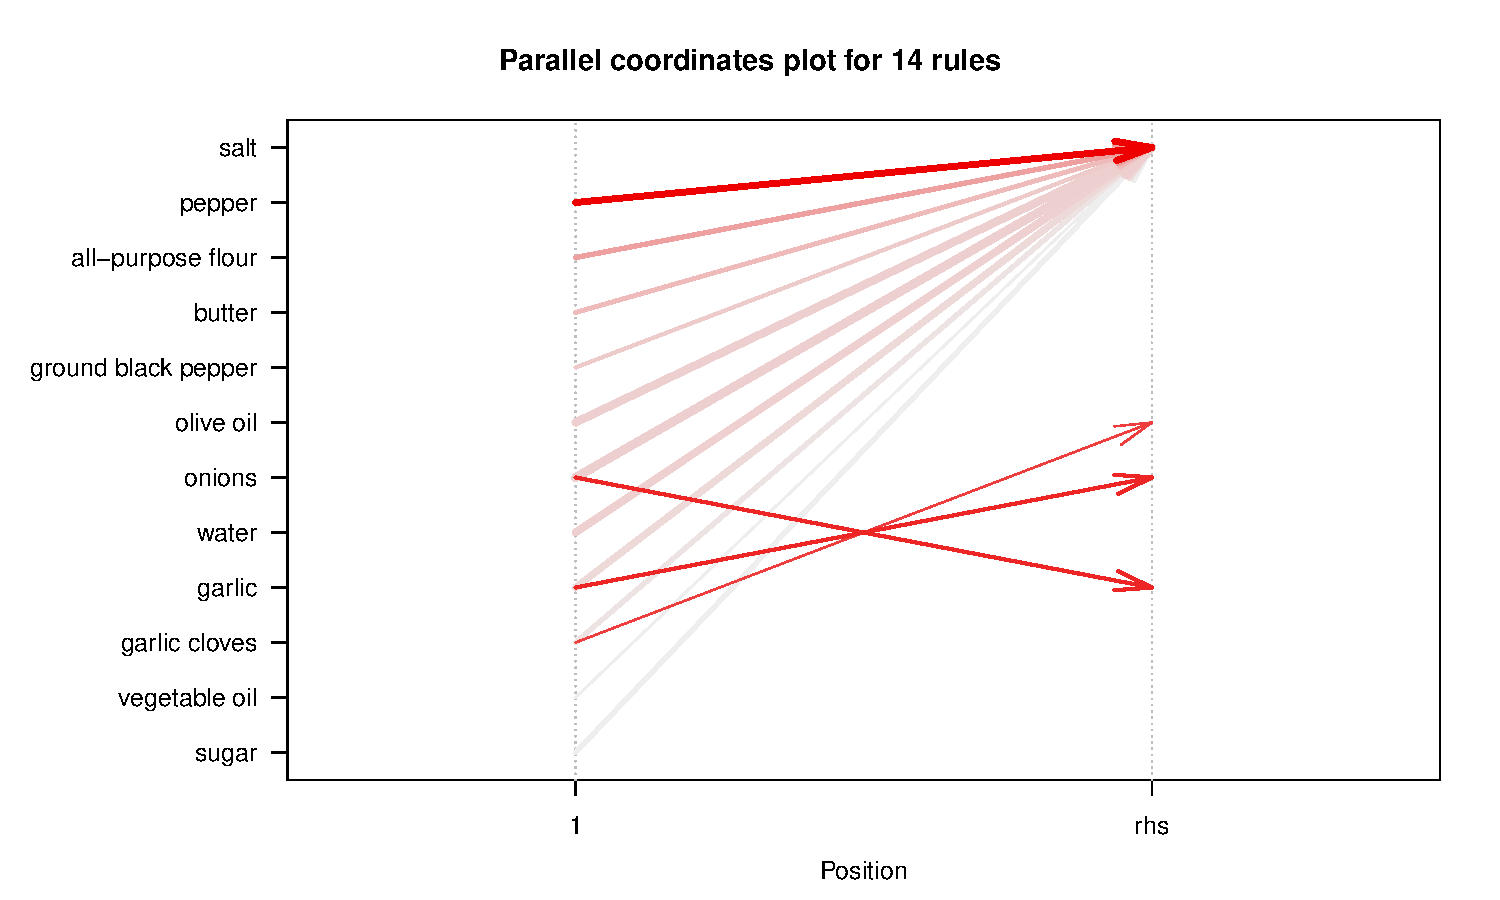
\includegraphics{Practica2-asociaciones}

\begin{Schunk}
\begin{Sinput}
> plot(asociaciones , method="grouped");
\end{Sinput}
\end{Schunk}
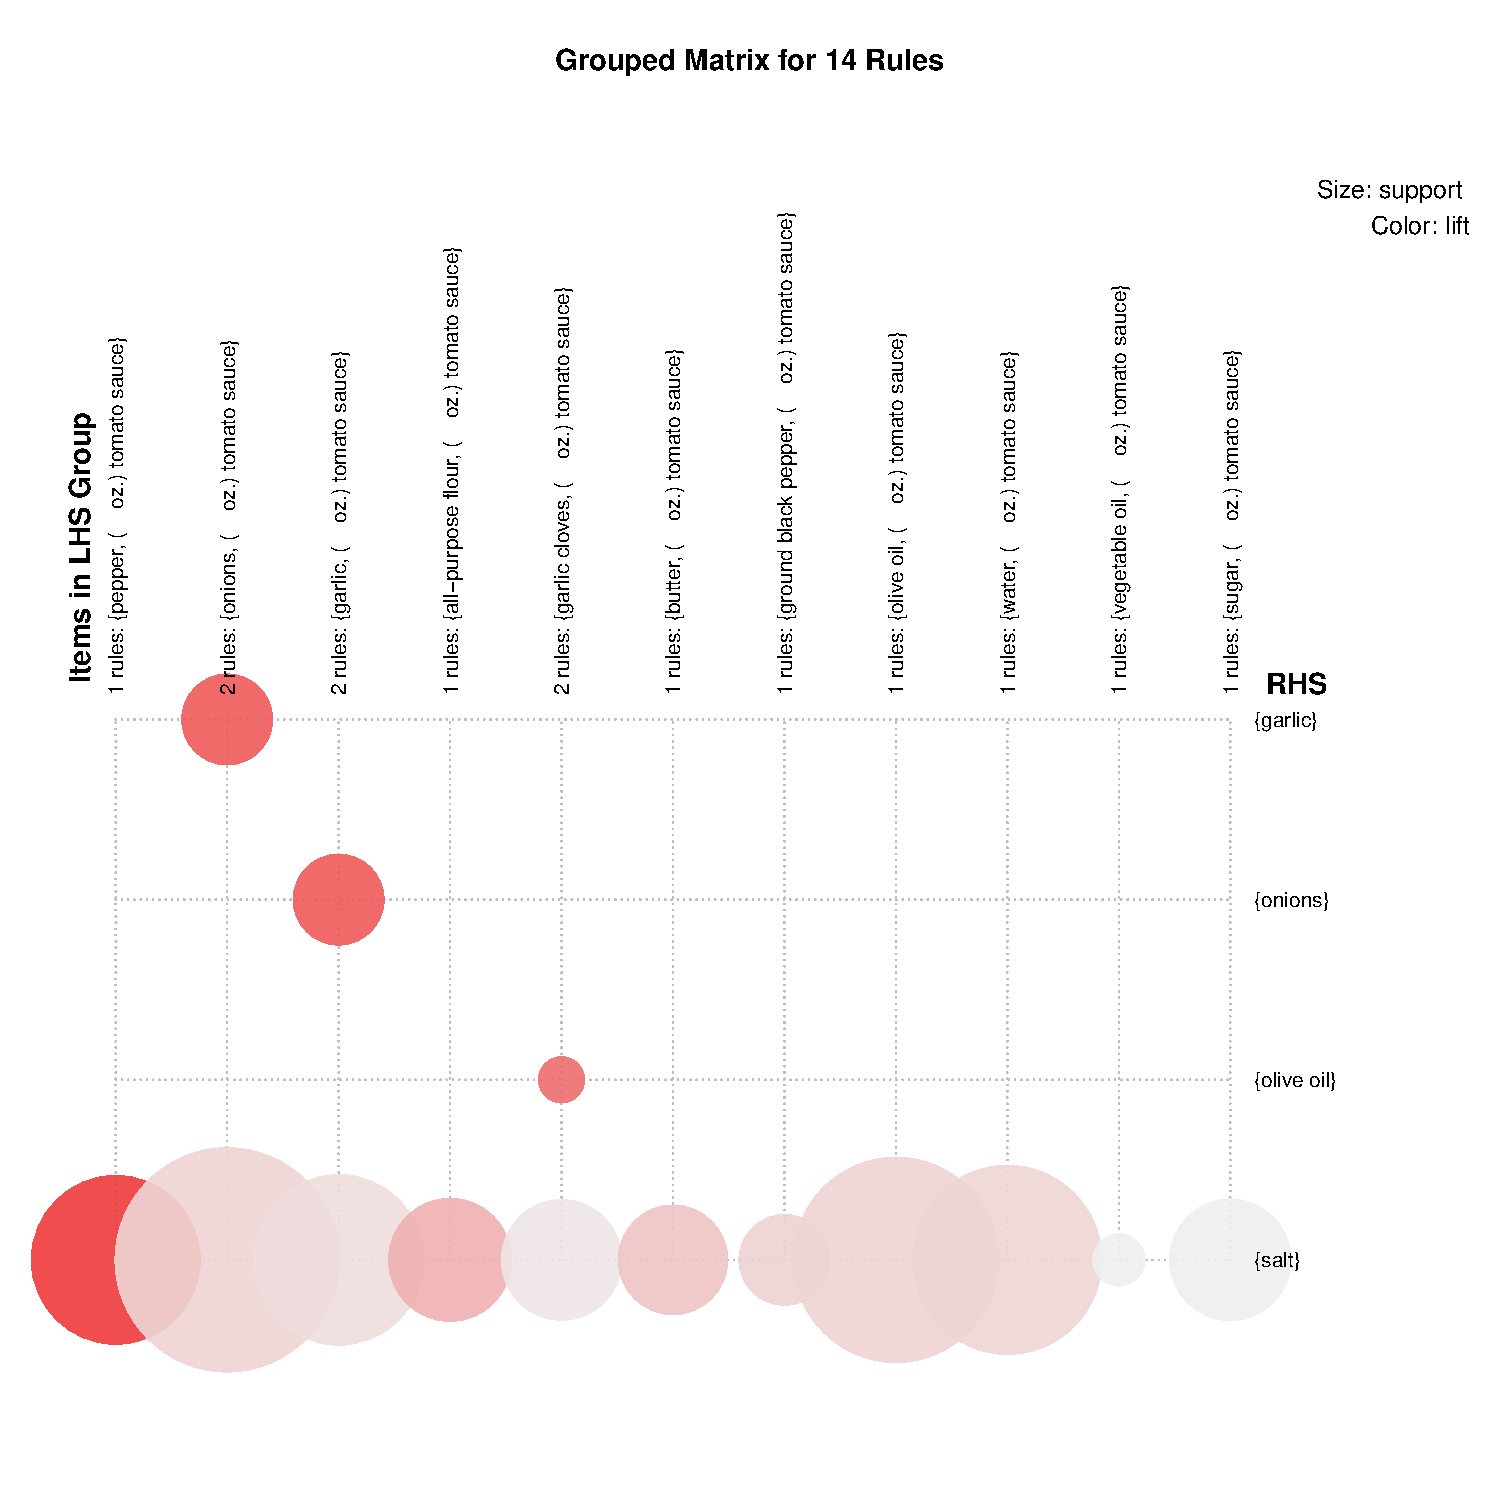
\includegraphics{Practica2-agrup1}
\begin{Schunk}
\begin{Sinput}
> plot(asociaciones, method = "graph")
\end{Sinput}
\end{Schunk}
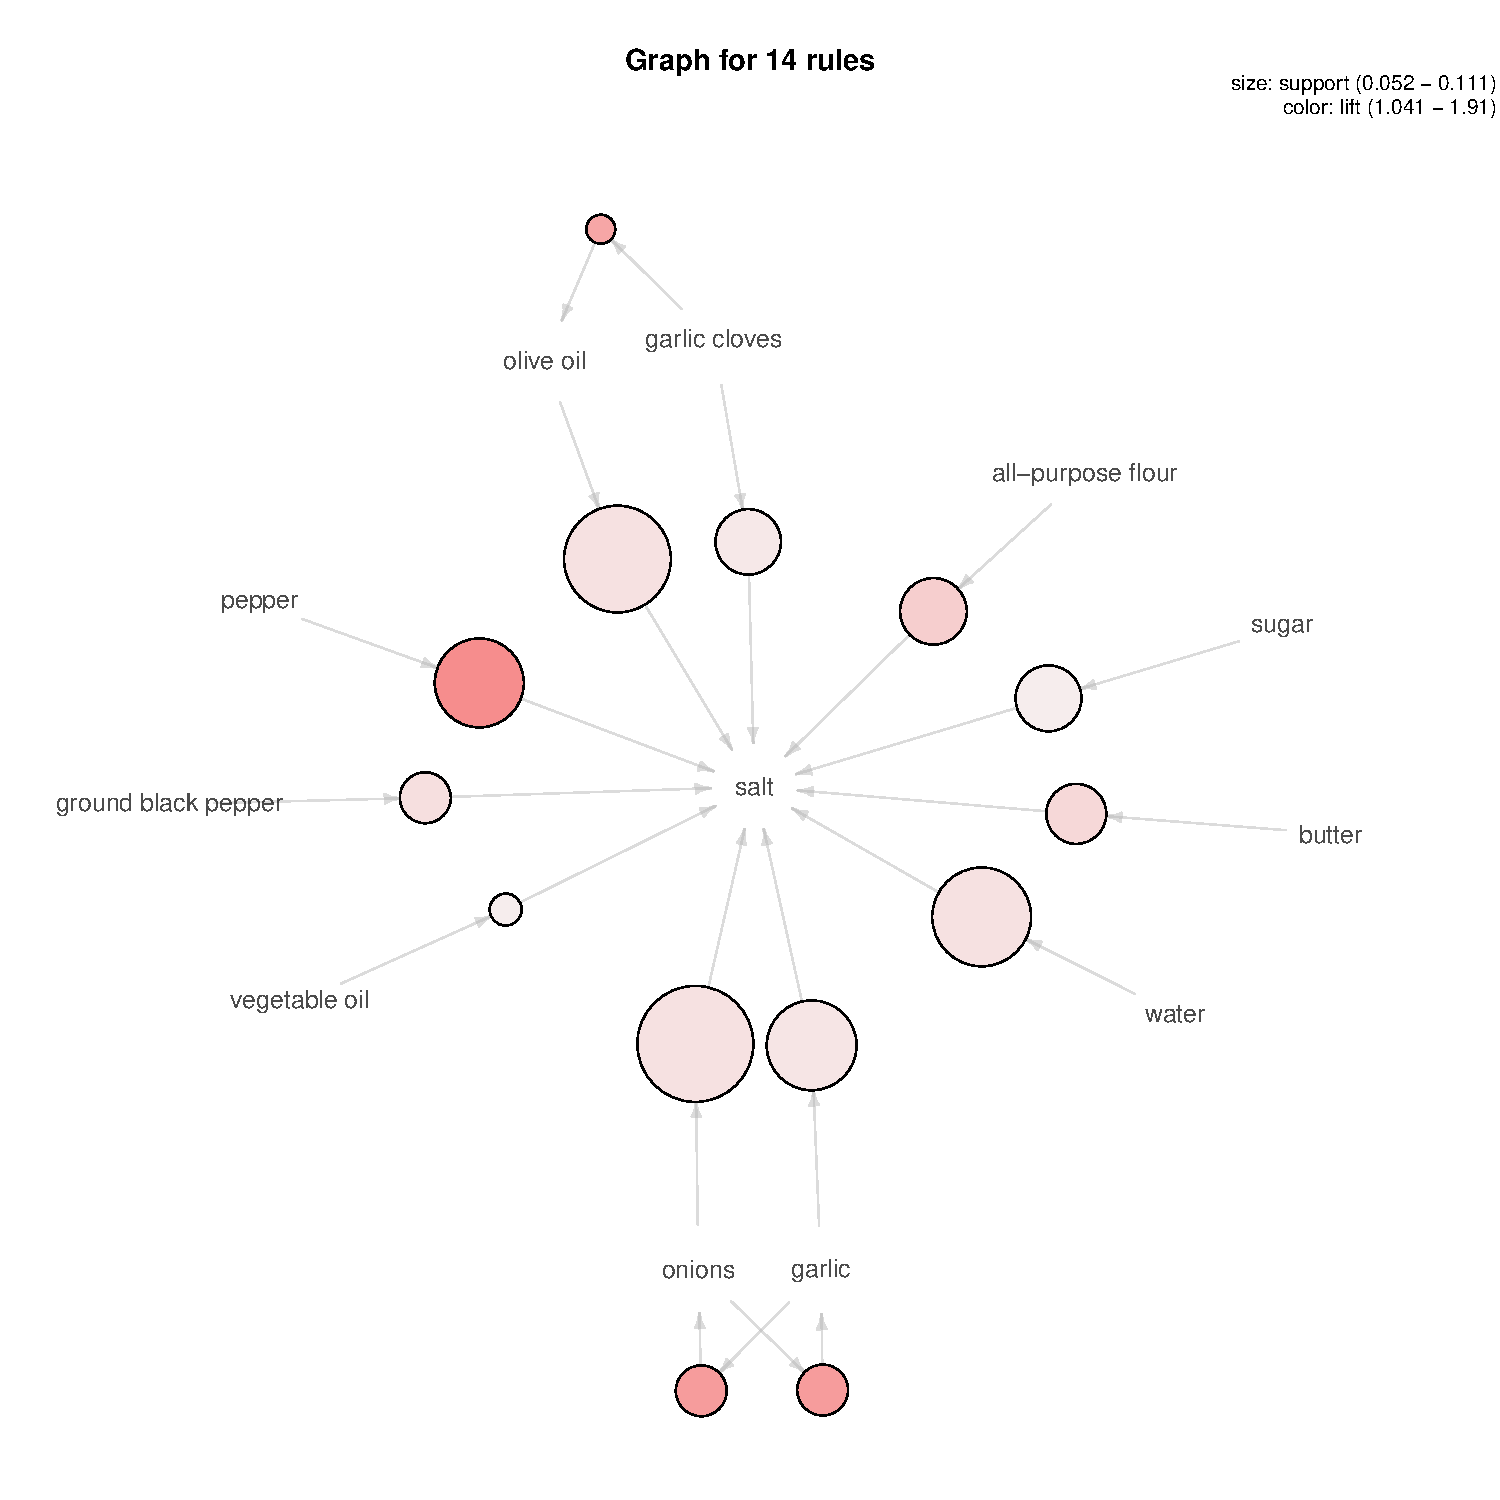
\includegraphics{Practica2-grafo1}
\begin{Schunk}
\begin{Sinput}
> plot(asociaciones )
\end{Sinput}
\end{Schunk}
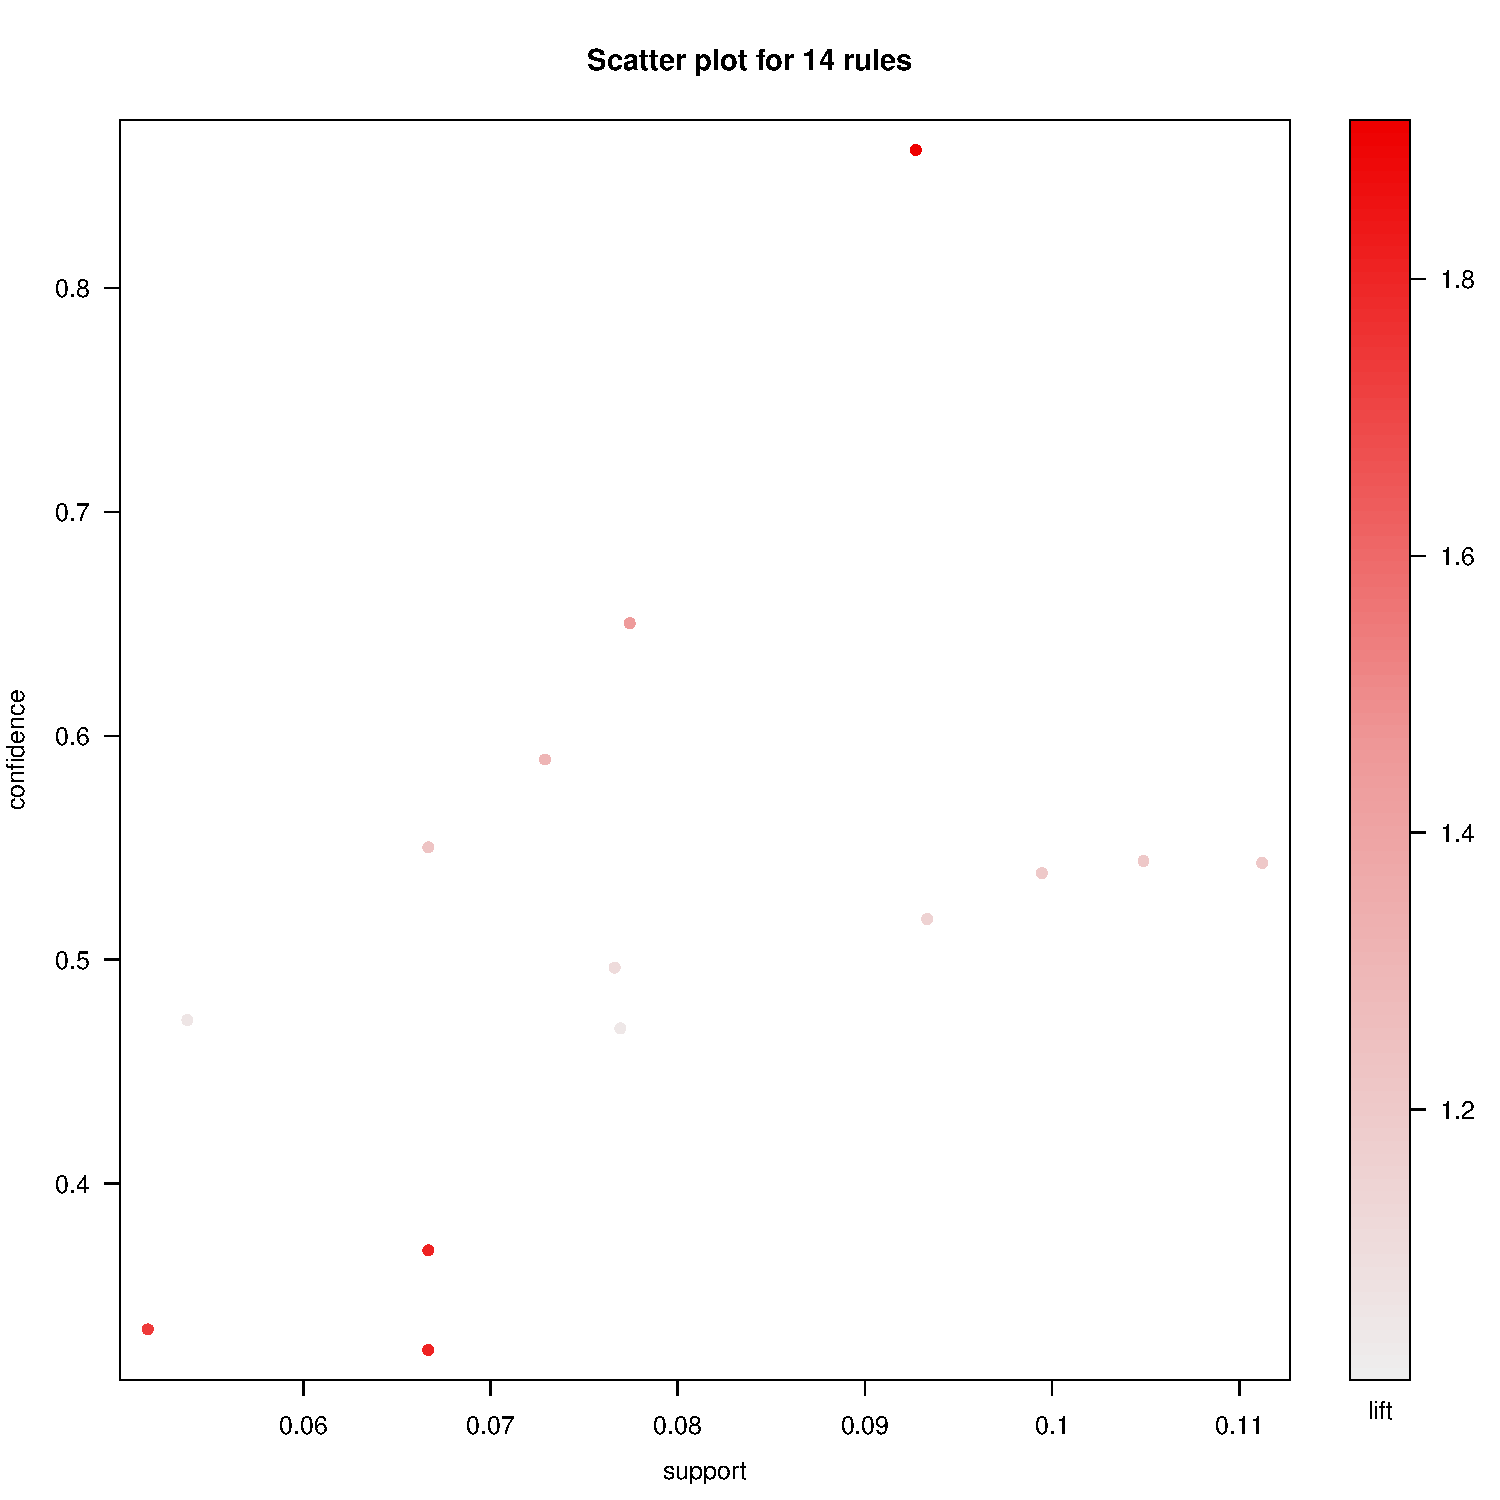
\includegraphics{Practica2-scatter1}
\begin{Schunk}
\begin{Sinput}
> plot(asociaciones , method="matrix",engine="3d", measure="lift");
\end{Sinput}
\begin{Soutput}
Itemsets in Antecedent (LHS)
 [1] "{pepper}"              "{onions}"              "{garlic}"             
 [4] "{all-purpose flour}"   "{garlic cloves}"       "{butter}"             
 [7] "{ground black pepper}" "{olive oil}"           "{water}"              
[10] "{vegetable oil}"       "{sugar}"              
Itemsets in Consequent (RHS)
[1] "{salt}"      "{olive oil}" "{onions}"    "{garlic}"   
\end{Soutput}
\end{Schunk}
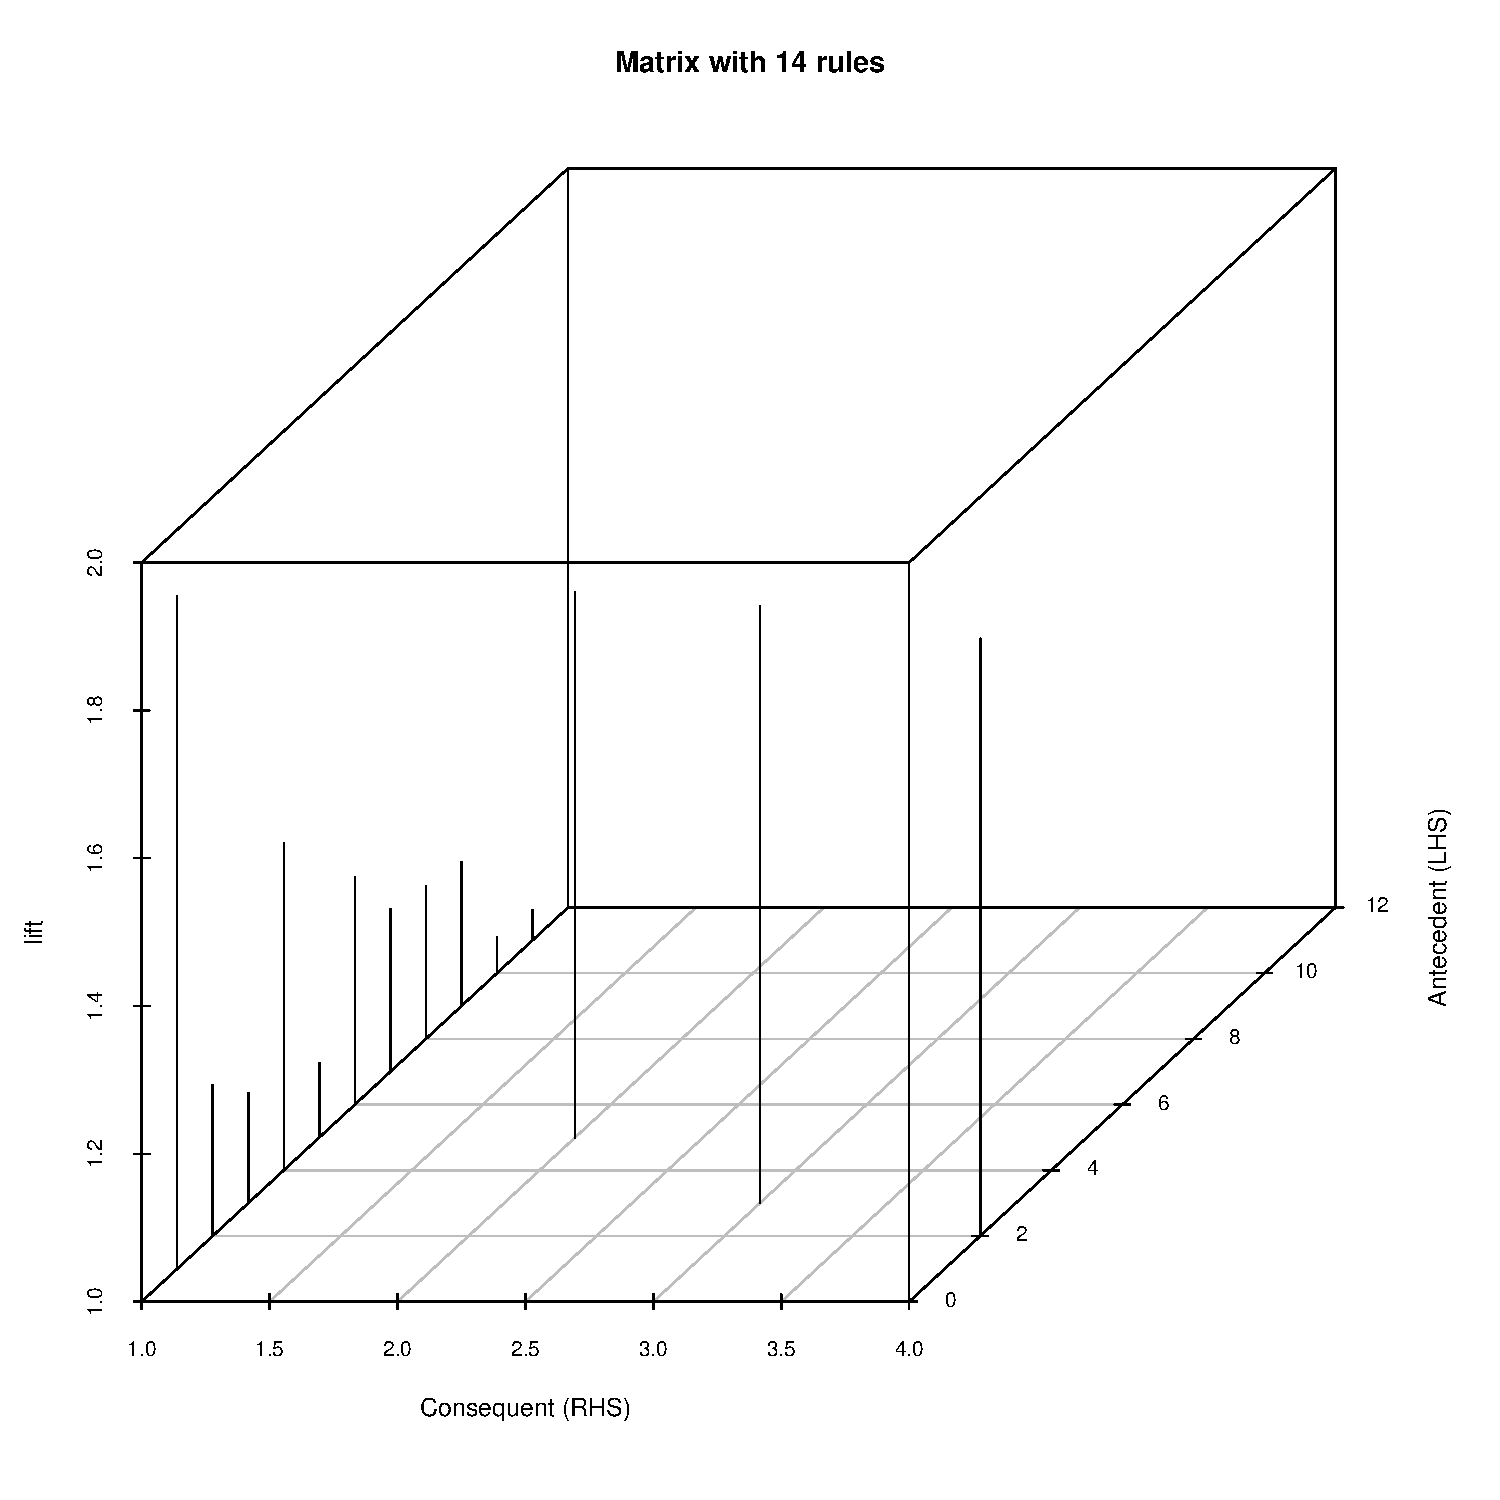
\includegraphics{Practica2-scatter3d1}
\begin{Schunk}
\begin{Sinput}
> plot(asociaciones , method = "graph",  engine = "htmlwidget")
\end{Sinput}
\end{Schunk}
\end{document}
